\documentclass[14pt]{article}

\usepackage[polish]{babel}
\usepackage[utf8]{inputenc}
\usepackage[T1]{fontenc}
\usepackage{extsizes}
\usepackage{graphicx}
\usepackage{tocloft}
\usepackage{amsmath}
\usepackage{multirow}
\usepackage{hyperref}


\font\titlefont=cmtt10 at 22pt

\title{
    
\includegraphics[scale=0.5]{images/logo-pwr-pion.png}
    \vspace{1cm}
    \\
    {\textbf{
    \titlefont Sygnały i obrazy cyfrowe
    \\ Laboratorium 2 - Skalowanie i rotacja
    }}
}
    
\author{
    Informatyczne Systemy Automatyki
    \\
    \\ Wykonujący:
    \\ Igor Potyrała - 272518
    \\
    \\ Prowadzący - Przemysław Śliwiński
}
\date{Data laboratoriów: 8 listopada oraz 25 pażdziernika 2023}


\begin{document}
\maketitle
\newpage
% Spis treści
%\newpage
%\renewcommand{\cftsecleader}{\cftdotfill{\cftdotsep}}
%{
 % \hypersetup{linkcolor=black, hidelinks}
 % \tableofcontents
%}

% Wstęp teoretyczny, definicje
\section{Zadania}
\subsection{Algorytmy interpolacji}
Celem zadania pierwszego było sprawdzenie działania 3 algorytmów interpolacji
do skalowania oraz obracania względem puntku. Algorytmy te to:
\begin{itemize}
    \item Najbliższy sąsiad,
    \item Liniowa,
    \item Sześcienna
\end{itemize}

\subsection{Skalowanie i rotacja}
\subsubsection{Wyniki}
\begin{center}
    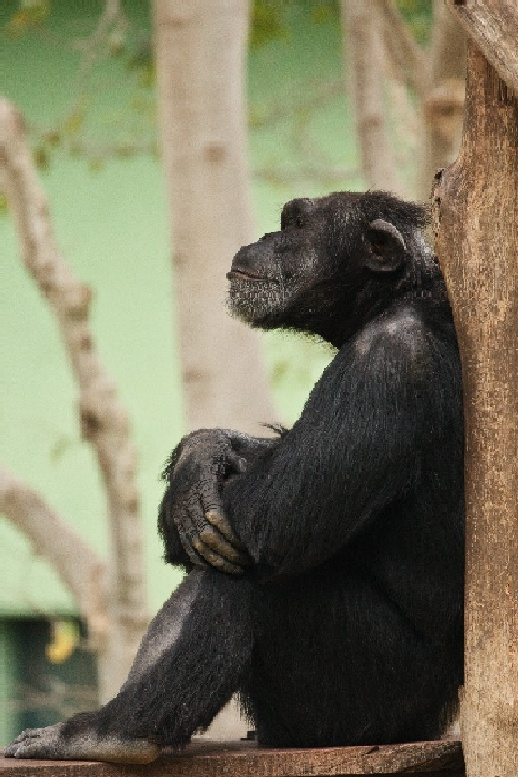
\includegraphics[scale=0.3]{images/5x_BACK_TO_ORG_nn.jpg}
    \\ \small Obraz 1. 5-krotne powiększenie o 10\%, a następnie pomniejszenie
    do oryginalnej wielkości - najbliższy sąsiad.

    \vspace{0.2cm}
    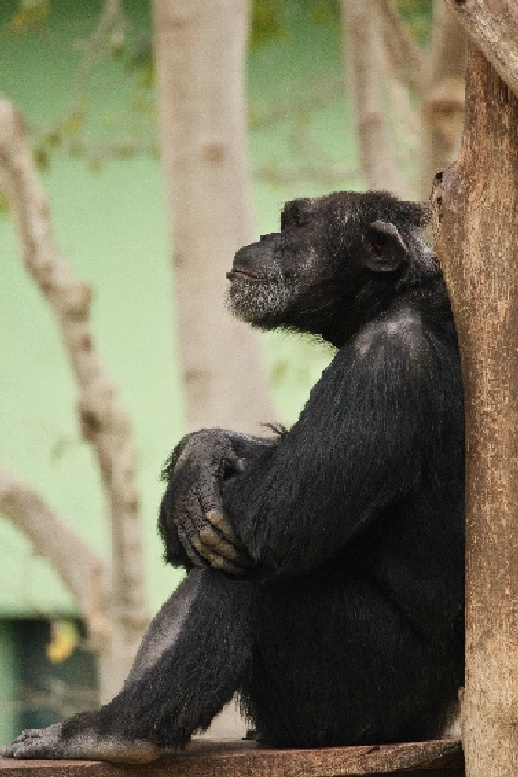
\includegraphics[scale=0.3]{images/3x_BACK_TO_ORG_nn.jpg}
    \\ \small Obraz 2. 3-krotne pomniejszenie o 10\%, a następnie powiększenie
    do oryginalnej wielkości - najbliższy sąsiad.

    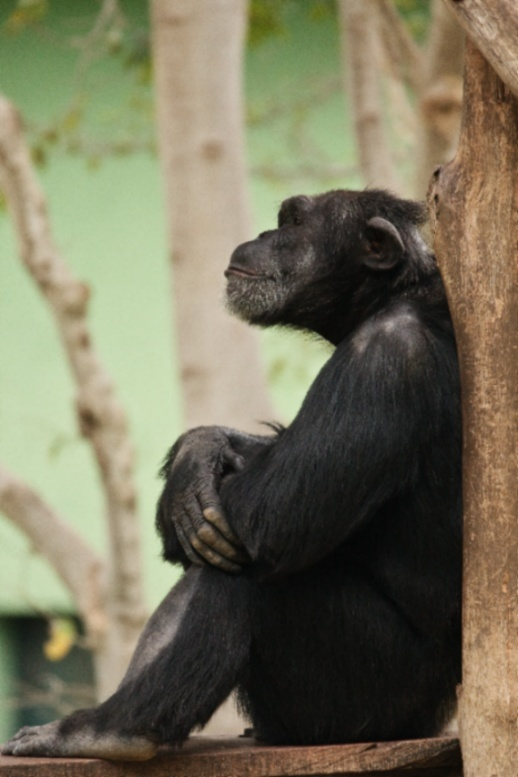
\includegraphics[scale=0.3]{images/5x_BACK_TO_ORG_bl.jpg}
    \\ \small Obraz 3. 5-krotne powiększenie o 10\%, a następnie pomniejszenie
    do oryginalnej wielkości -liniowa.

    \vspace{0.2cm}
    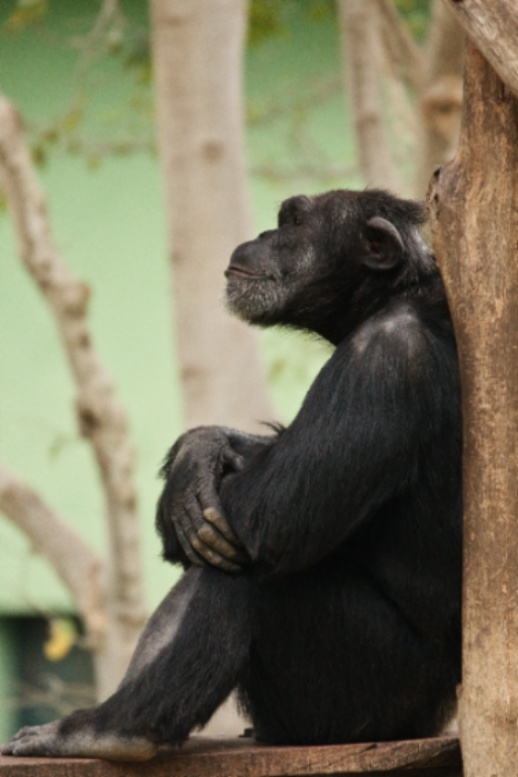
\includegraphics[scale=0.3]{images/3x_BACK_TO_ORG_bl.jpg}
    \\ \small Obraz 4. 3-krotne pomniejszenie o 10\%, a następnie powiększenie
    do oryginalnej wielkości - liniowa.

    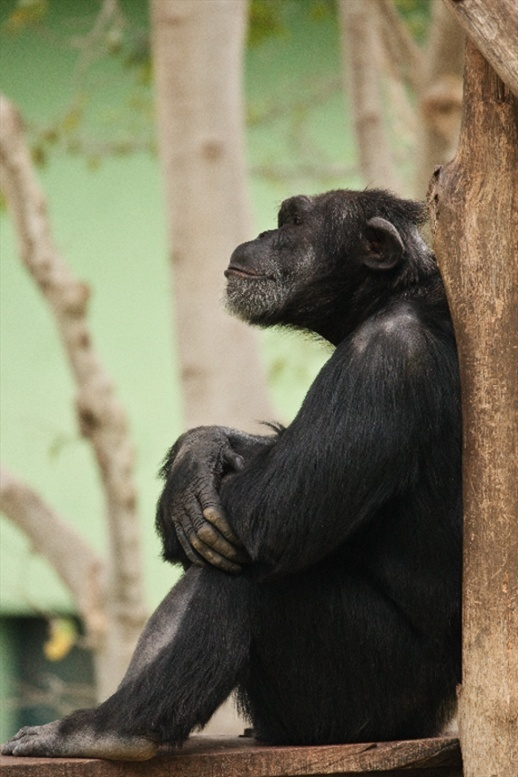
\includegraphics[scale=0.3]{images/5x_BACK_TO_ORG_bc.jpg}
    \\ \small Obraz 5. 5-krotne powiększenie o 10\%, a następnie pomniejszenie
    do oryginalnej wielkości - sześcienna.

    \vspace{0.2cm}
    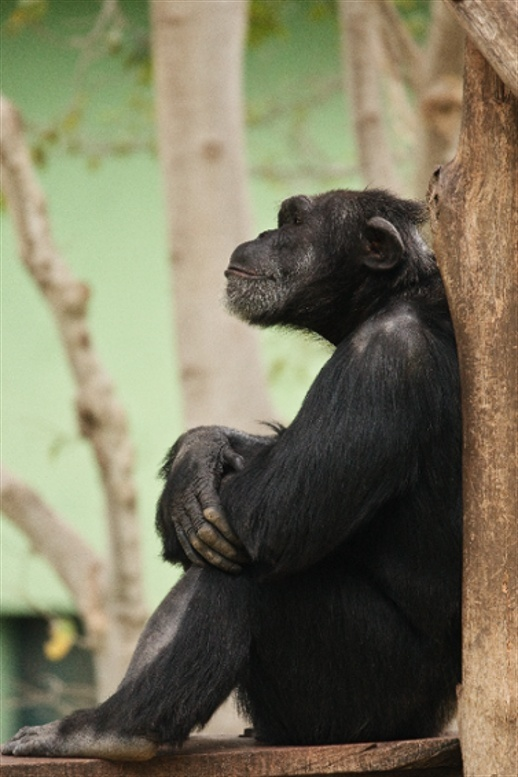
\includegraphics[scale=0.3]{images/3x_BACK_TO_ORG_bc.jpg}
    \\ \small Obraz 6. 3-krotne pomniejszenie o 10\%, a następnie powiększenie
    do oryginalnej wielkości - sześcienna.

    \vspace{0.25cm}
    \begin{tabular}{|c|c|c|c|}
        \hline
        %\multicolumn{3}{|c|}{Dokładność pomiarów napięcia DC}\\ 
        %\cline{1-3}
        %\hline
        & Najbliższy sąsiad & Liniowa & Sześcienna  \\ \hline
        Powiększenie & 0,38s & 4,86s & 55,35s \\ \hline
        Pomniejszenie & 0,27s & 2,77s & 40,51s \\ \hline
        Średni błąd kwadratowy & 55,41 & 33,10 & 23,37 \\ \hline

    \end{tabular}
    \vspace{0.2cm}
    \\ \small Tabela 1. Przedstawiające charakterystyki 
    czasowe oraz błędy typów interpolacji.
\end{center}
\subsubsection{Wnioski}

\newpage
\section{Wnioski}
Zakłócenia ukazujące się w obrazie 3 wynikają z 
niespełnienia warunków twierdzenia o próbkowaniu. Obiekt
porusza się zbyt szybko, by macierz sensora zarejestrowała 
wszystkie piksele. Przykładowe sposoby na zniwelowanie 
tego efektu:
\vspace{0.25cm}
\begin{itemize}
    \item Unikanie ruchu podczas filmowania / trzymanie kamery 
    nieruchomo zminimalizuje zniekształcenia,
    \item Zwiększenie prędkości odczytu sensora, by była 
    większa od prędkości obracania się łopatek.
\end{itemize}

\vspace{0.25cm}
* Uniwersalną funkcją może być ta ,którą użyliśmy w poprzednich zadaniach,
$f(x) = sin(nx + \frac{m\pi}{RPM})$, wystarczy zmieniać tylko
parametr $n$ w zależności od tego ile śmigieł chcemy. Przy większej 
ilości łopatek warto będzie, także zwiększyć wielkość generowanego obrazu.
\end{document}